%!TEX root=./main.tex


%By contrast, our approach uses \emph{several laparoscopic images simultaneously} (usually at least $4$) to perform the initial registration.  We show how to use multiple viewpoints of a mobile organ to obtain considerably more surface information and therefore a more accurate registration. Moreover, our method is the first to integrate \emph{occluding contour fragments} as additional registration constraints.

%The approach has been tested in the case of the uterus but it is easily adaptable to other organs and other pre-operative 3D modalities.



\section{Methodology}
% \vspace{-0.05in}
% \subsection{Section Overview}
\label{sec:ARGuidanceSystem}
%We first describe the system's requirements regarding pre-operative data (\sect{sec:inputModels}) and then a global overview of the intra-operative registration process (\sect{sec:globalOverview}). We then describe the two main components of registration, which are the \emph{initial registration} and \emph{tracking} stages (\sect{sec:initialRegistration} and \sect{sec:updateRegistration}, respectively). %CARE:Lastly we present Tool Access Visualisation (\sect{sec:toolPortProj}). 
\begin{figure}[t]
	\centering
	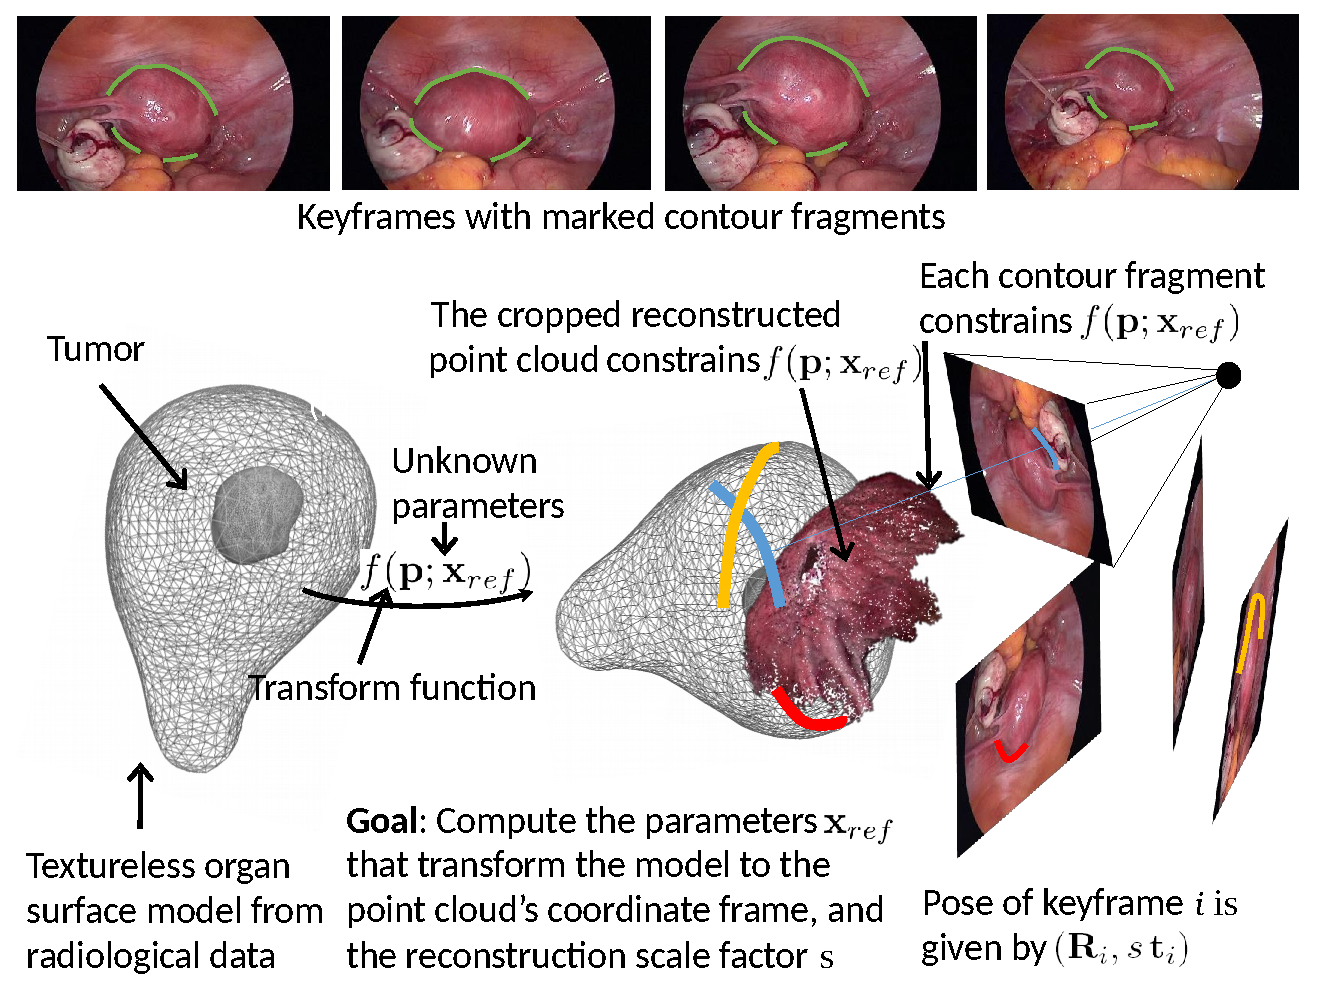
\includegraphics[width=0.8\columnwidth]{./figs/reconstructionDemoNew.pdf}
	\caption{The initial registration problem illustrated on a patient case. Four keyframes from the exploratory video are shown in the first row with their associated silhouette contour fragments.}
	\label{fig:initialRegOverview}
\end{figure}

\subsection{Pre-operative Data Requirements}
\label{sec:inputModels}
The system requires a segmented pre-operative 3D organ model, which comprises the organ's surface mesh, and meshes of internal structures to be visualized with AR.
For the uterus, internal structures are typically the cavity, tumors and safe-tissue margins. %Here the internal structures are tumors and their \emph{safe tissue margin}.
%A safe tissue margin is a border around the tumor of healthy tissue which should also be removed, whose thickness $w$ depends on the risk factor of the particular tumor.
Our approach does not require a specific organ deformation model to be used, because to date there is no clear consensus on the best one to use for registering organs. %Models currently range from complex heterogeneous mechanical models to simpler homogeneous algebraic models such as As-Rigid-As-Possible \cite{Sorkine:2007:ASM:1281991.1282006}. 

We require two interfaces to the deformation model. 
The first is the \emph{transform function} $f(\vet{p};\vet{x}_t): \Omega\rightarrow \mathbb{R}^3$.
Given the model's parameters $\vet{x}_t$ at time $t$, it transforms a 3D point $\vet{p}$ of the model's 3D domain $\Omega\subset \mathbb{R}^3$ to the laparoscope coordinate frame. 
The second interface is the internal energy function $\Einternal(\vet{x}_{t}):\mathbb{R}^{d}\rightarrow\mathbb{R}^{+}$. This returns the internal energy for transforming the organ according to $\vet{x}_t$ (for mechanical models, the strain energy induced by soft-tissue deformation), used to regularize the deformation.
% We require two interfaces to the deformation model. The first is the \emph{transform function} $f(\vet{p};\vet{x}_t): \Omega\rightarrow \mathbb{R}^3$: it is used to transforms a 3D point $\vet{p}$ of the model's 3D domain $\Omega\subset \mathbb{R}^3$ to the target coordinate frame (in our case, the laparoscope coordinates frame). The vector $\vet{x}_t$ denotes the model's parameters at time $t$. %The registration problem is  to determine $\vet{x}_t$ given a laparoscopic image at time $t$. 
% The second is the internal energy function $\Einternal(\vet{x}_{t}):\mathbb{R}^{d}\rightarrow\mathbb{R}^{+}$ which gives the internal energy for transforming the organ with $\vet{x}_t$, where $d$ is the dimensionality of $\vet{x}_{t}$. 
We only require that $f$ and $\Einternal$ be continuously differentiable, which is satisfied by virtually all models of interest.
%We describe the specific deformable models used in our experiments in Section \ref{sec:experiments_Simulation}.
 
\subsection{Registration Pipeline Overview}
\label{sec:globalOverview}
Our task is registration, to compute $\vet{x}_t$ for a given live monocular laparoscopic image. 
We break it down into the \textit{initial registration stage} and the \emph{tracking stage}. 
The initial registration is important for two main reasons. Firstly, the different patient posture between pre-operative and intra-operative steps and the insufflation may induce a significant deformation of the organ. Initial registration estimates this change of shape from the pre-operative to the intra-operative state, or \emph{reference state}. 
Secondly, during the tracking stage, we assume that the organ does not undergo significant deformations so that the tracking stage can be reasonably modeled with rigid motion.  The initial registration allows us to associate texture with the organ's surface, necessary to achieve tracking.
% The purpose of the initial registration stage is two-fold. Firstly, it estimates the change of shape of the organ between its pre-operative state and an intra-operative state, called the \emph{reference state}, caused by physiological movement between pre-operative and intra-operative states, such as patient posture difference and insufflation. Secondly, it associates texture with the organ's surface, which is required in the tracking stage.
% To achieve high robustness we make a simplifying assumption in the tracking stage, which is that the organ does not deform significantly during this stage.
% To simplify the problem, we assume that during the tracking stage the organ does not deform significantly. Therefore, the tracking stage can be modelled with rigid motion, which can be estimated far more quickly and robustly than deformable motion. 

Formally, the two stages of registration break down $f(\vet{p};\vet{x}_t)$ as $f(\vet{p};\vet{x}_{t})=M(f(\vet{p};\xref);\mat{R}_{t},\vet{t}_{t})$. Here \xref denotes the organ's unknown deformation for the reference state.
The function $M(\cdot;\mat{R}_{t},\vet{t}_{t}):\mathbb{R}^3\rightarrow \mathbb{R}^3$ denotes the unknown update transform at time $t$, parameterized by a 3D rotation $\mat{R}_{t}\in \mathcal{SO}_{3}$ and translation $\vet{t}_{t}\in \mathbb{R}^3$.
%Thus, the initial registration stage estimates $\vet{x}_{ref}$ and the tracking stage estimates $(\mat{R}_{t},\vet{t}_{t})$.

In practice, the rigidity assumption during tracking is reasonable because during live AR guidance the surgeon does not significantly deform the organ.
% In practice, rigidity during tracking is a good assumption when the surgeon does not significantly deform the organ during the tracking stage (\ie the period that they wish to use live AR guidance). 
We emphasize that the intended use of AR is to assist spatial comprehension of internal structures and intra-operative resection planning. Typically this is done by guiding the marking of a tumor resection plane on the uterus surface with a coagulation instrument. Such marking is standard practice in uterine surgery. During the actual resection, AR visualization is deactivated because the surgeon follows the coagulation marks.

To provide real-time AR, only the tracking stage needs to be real-time. To minimize workflow interruption, we require the initial registration to be computed in no longer than a few minutes. 
The manual pre-processing takes on average $\SI{2}{\minute}$ and the optimisation $\SI{1}{\minute}$.
% With our current implementation this takes approximately three minutes on a standard workstation PC (approximately two minutes for manual pre-processing and one minute for optimisation). 
Tracking is an optimized implementation in \CC/CUDA and runs at $\sim\SI{25}{fps}$.